\documentclass[11pt]{article}
\usepackage[normalem]{ulem}
\usepackage{fancyhdr}
\RequirePackage{etex}
\usepackage{amsmath, amssymb, amsfonts}
\usepackage{tikz}
\usetikzlibrary{arrows,shapes,automata,positioning,backgrounds,petri}
\usepackage{tcolorbox}
\usepackage{tikz-network}

\setlength{\oddsidemargin}{12pt}
\setlength{\textwidth}{6.5in}
\setlength{\textheight}{8in}
\setlength{\headheight}{14pt}
\setlength{\parskip}{7pt plus 2pt minus 2pt}
\pagestyle{fancy}
\renewcommand{\headrulewidth}{0pt}
\markright{\textbf{ComS 331 \hspace{20pt} Spring 2025 \hspace{20pt} Name:} \dashuline{Pranava Sai Maganti}}

\begin{document}

\begin{center}
    \textbf{HW 0 \hspace{15pt} Due: 28 jan 2025}
\end{center}

\begin{enumerate}
    \item \textbf{Answer}:
    \tcbset{colframe=black, colback=white, boxrule=0.5pt, arc=0pt, width=6in, auto outer arc}
    \begin{tcolorbox}
        This is an inline equation: $x + y = 3$. \\
        This is a displayed equation:
        \[
        x + \frac{y}{z - \sqrt{3}} = 2.
        \]
        This is how you can define a piece-wise linear function:
        \[
        f(x) =
        \begin{cases} 
                3x + 2 & \text{if } x < 0 \\
                7x + 2 & \text{if } x \geq 0 \text{ and } x < 10 \\
                5x + 22 & \text{otherwise}.
        \end{cases}
        \]
        This is a matrix:
        \begin{center}
            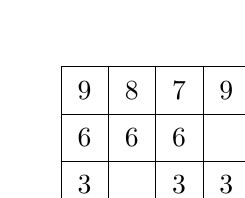
\begin{tikzpicture}
                \draw[step=0.6cm, ultra thin] (0,0) grid (2.4,1.8);
            
                \node at (0.3,1.5) {9};
                \node at (0.9,1.5) {8};
                \node at (1.5,1.5) {7};
                \node at (2.1,1.5) {9};
            
                \node at (0.3,0.9) {6};
                \node at (0.9,0.9) {6};
                \node at (1.5,0.9) {6};
                \node at (2.1,0.9) {};
            
                \node at (0.3,0.3) {3};
                \node at (0.9,0.3) {};
                \node at (1.5,0.3) {3};
                \node at (2.1,0.3) {3};
            \end{tikzpicture}
        \end{center}

        
        This is a graph with two types (solid and dashed) of labeled edges:
        
        \begin{center}
        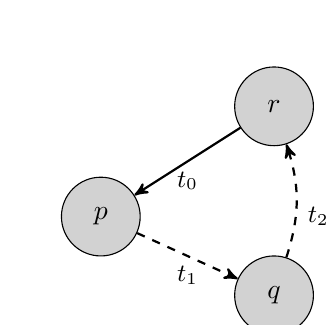
\begin{tikzpicture}[node distance=6ex and 10ex,->,>=stealth',bend angle=15,auto]
            \node[draw, circle, minimum size=1cm, fill=lightgray!70] (p) at (0, 0) {$p$};
            \node[draw, circle, minimum size=1cm, fill=lightgray!70] (r) at (2.2, 1.4) {$r$};
            \node[draw, circle, minimum size=1cm, fill=lightgray!70] (q) at (2.2, -1) {$q$};
            
            \draw[->, solid, thick] (r) -- (p) node[midway, below, font=\small] {$t_0$};
            \draw[->, dashed, thick] (p) -- (q) node[midway, below, font=\small] {$t_1$};
            \draw[->, dashed, thick, bend right=18] (q) to (r) 
                node[midway, right=25mm, font=\small] {$t_2$};
        \end{tikzpicture}
        \end{center}
        \end{tcolorbox}

    \item \textbf{Answer}:\\
    \uline{Given}: A set of $\mathbb{N} = \{0,1,2,3,4,...\}\ $ and a set of $\mathbb{Z} = \{...,-2,-1,0,1,2,...\}\ $

    \uline{To Prove}: There exists a bijection $ f: \mathbb{N} \rightarrow \mathbb{Z} $, demonstrating that $ \mathbb{N} $ and $ \mathbb{Z} $ are equinumerous.

    \uline{Proof}:
    We first start of by defining the piecewise functions as follows:\\
    \[
        f(n) =
        \begin{cases} 
                0 & \text{if } n = 0 \\
                \frac{n+1}{2} & \text{if } n\mod2\neq 0\\
                \frac{-n}{2} & \text{if } n\mod2=0\\
        \end{cases}
    \]
    Here the function $f(n)$ is the piecewise function, where $n \in \mathbb{N}$.
    Next, we will have prove that the defined function $f(n)$ is both \textbf{one-to-one} and \textbf{onto}.

\begin{enumerate}
    \item \textbf{$ f $ is One-to-One} \\
To prove $ f $ is one-to-one, let's assume $ f(n_1) = f(n_2) $ for some $ n_1, n_2 \in \mathbb{N} $.  
We consider two cases based on the parity (even or odd) of $ n_1 $ and $ n_2 $:

\begin{enumerate}
    \item \textbf{Case 1: Both $ n_1 $ and $ n_2 $ are even.} \\
If $ n_1 = 2k_1 $ and $ n_2 = 2k_2 $, then: \\
\\
$f(n_1) = \frac{-n_1}{2} = \frac{-2k_1}{2} = -k_1$ \\
\\
Similarly, $f(n_2) = \frac{-n_2}{2} = \frac{-2k_2}{2} = -k_2$\\
\\
Since $ f(n_1) = f(n_2) $, we have $-k_1 = -k_2 \implies k_1 = k_2$, which in-turn implies that $n_1 = n_2$. \\

\item \textbf{Case 2: Both $ n_1 $ and $ n_2 $ are odd.} \\
If $ n_1 = 2k_1 + 1 $ and $ n_2 = 2k_2 + 1 $, then: \\
\\
$f(n_1) = \frac{n_1+1}{2} = \frac{2k_1+2}{2} = \frac{2(k_1+1)}{2} = k_1$ \\
\\
Similarly, $f(n_2) = \frac{n_2+1}{2} = \frac{2k_2+2}{2} = \frac{2(k_2+1)}{2} = k_2$ \\

Since $ f(n_1) = f(n_2) $, we have $k_1 + 1 = k_2 + 1 \implies k_1 = k_2$
which implies $ n_1 = n_2 $. \\

\item \textbf{Case 3: $ n_1 $ is even and $ n_2 $ is odd (or vice versa).} \\
If $ n_1 $ is even, $ f(n_1) \leq 0 $.  
If $ n_2 $ is odd, $ f(n_2) > 0 $.  
Therefore, $ f(n_1) \neq f(n_2) $.
\end{enumerate}

Since $ f(n_1) = f(n_2) $ implies $ n_1 = n_2 $ in all cases, $ f $ is one-to-one.
\\
\item \textbf{$ f $ is Onto} \\
To prove $ f $ is onto, we show that for every $ z \in \mathbb{Z} $, there exists $ n \in \mathbb{N} $ such that $ f(n) = z $.
\begin{enumerate}
    \item \textbf{Case 1: $ z \leq 0 $.} \\
Let $ n = -2z $. Since $ z \leq 0 $, $ -2z \geq 0 $, so $ n \in \mathbb{N} $.  
For this $ n $,
\[
f(n) = -\frac{n}{2} = -\frac{-2z}{2} = z.
\]

\item \textbf{Case 2: $ z > 0 $.} \\
Let $ n = 2z - 1 $. Since $ z > 0 $, $ n = 2z - 1 \geq 0 $, so $ n \in \mathbb{N} $.  
For this $ n $,
\[
f(n) = \frac{n+1}{2} = \frac{(2z - 1) + 1}{2} = z.
\]

Thus, for every $ z \in \mathbb{Z} $, we can find $ n \in \mathbb{N} $ such that $ f(n) = z $. Therefore, $ f $ is onto.
\end{enumerate}

Since $ f $ is both one-to-one and onto, it is a bijection.

\end{enumerate}
\pagebreak

\item \textbf{Answer}: \\
\uline{Given:}  
A relation $ R $ on $ \mathbb{N} $ defined by:  \\
    $\forall m, n \in \mathbb{N}, (m, n) \in R \iff (m - n) \mod 3 = 0$

\uline{To Prove:}  
\begin{enumerate}
    \item $ R $ is an equivalence relation (i.e., $ R $ is reflexive, symmetric, and transitive).  
    \item Describe the equivalence classes of $ R $.
\end{enumerate}

\uline{Proof:}
\begin{enumerate}
    \item \textbf{Reflexive:}  
   For any $ m \in \mathbb{N} $, $ m - m = 0 $, and $ 0 \mod 3 = 0 $.  \\
   Hence, $ (m, m) \in R $. \\ 
   Therefore, $ R $ is reflexive.
    \item \textbf{Symmetric:}  
   Let $ (m, n) \in R $. This means $ (m - n) \mod 3 = 0 $.  \\
   Then, $ m - n = 3k $ for some $ k \in \mathbb{Z} $.  \\
   Rearranging$ n - m = -3k $, and since $ -3k \mod 3 = 0 $, we have $ (n, m) \in R $.  \\
   Therefore, $ R $ is symmetric.
    \\
    \item \textbf{Transitive:}  
   Let $ (m, n) \in R $ and $ (n, p) \in R $.  
   This means $ (m - n) \mod 3 = 0 $ and $ (n - p) \mod 3 = 0 $.  
   Then, $ m - n = 3k $ and $ n - p = 3l $ for some $ k, l \in \mathbb{Z} $.  
   Adding these equations, $ m - p = 3k + 3l = 3(k + l) $.  
   Hence, $ (m - p) \mod 3 = 0 $, so $ (m, p) \in R $.  
   Therefore, $ R $ is transitive.
\end{enumerate}

Since $ R $ is reflexive, symmetric, and transitive, $ R $ is an equivalence relation.

\textbf{Equivalence Classes:}  
Two numbers $ m, n \in \mathbb{N} $ are equivalent under $ R $ if $ (m - n) \mod 3 = 0 $.  
Thus, the equivalence classes are determined by the remainder when dividing a number by 3:  
\[
[0] = \{ n \in \mathbb{N} \mid n \mod 3 = 0 \}, \quad \text{i.e., } \{ 0, 3, 6, 9, \cdots \}
\]
\[
[1] = \{ n \in \mathbb{N} \mid n \mod 3 = 1 \}, \quad \text{i.e., } \{ 1, 4, 7, 10, \cdots \}
\]
\[
[2] = \{ n \in \mathbb{N} \mid n \mod 3 = 2 \}, \quad \text{i.e., } \{ 2, 5, 8, 11, \cdots \}
\]

Therefore, the equivalence classes are:  
$[0], [1], [2]$
\pagebreak
\item \textbf{Answer}: \\
\uline{To Prove}: \\
\begin{equation*}
    \sum_{i=1}^{n} i^2 = \frac{(2n + 1)(n+1)n}{6}
\end{equation*}

\uline{Proof}: \\
\begin{enumerate}
    \item \textbf{Base Case}:\\
    For $n = 1$ on LHS:
    \begin{equation*}
        \sum_{i=1}^{n} i^2 = 1
    \end{equation*}
    For $n = 1$ on RHS:
    \begin{equation*}
        \frac{(2(1) + 1)((1)+1)(1)}{6} = \frac{(2+1)(1+1)(1)}{6} = \frac{3*2*1}{6} = \frac{6}{6} = 1
    \end{equation*}
    Since LHS = RHS, base case holds true.
    
    \item \textbf{Inductive Hypothesis}:
    Assuming that the formula holds true for $n = k$:
    \begin{equation*}
        \sum_{i=1}^{k} i^2 = \frac{(2k+1)(k+1)k}{6}
    \end{equation*}
    \item \textbf{Inductive Step}:
    For the inductive step, we need to prove that the formula holds true for $n = k + 1$ also.
    For $n = k+1$: \\
    \begin{equation*}
        \sum_{i=1}^{k+1} i^2 = \frac{(2(k+1)+1)((k+1)+1)(k+1)}{6}
    \end{equation*}

    Simplifying on the LHS:
    \begin{equation*}
        \sum_{i=1}^{k+1} i^2 = \sum_{i=1}^{k} i^2 + (k+1)^2
    \end{equation*}
    From the inductive hypothesis, we know that:
    \begin{equation*}
        \sum_{i=1}^{k} i^2 = \frac{(2k+1)(k+1)k}{6}
    \end{equation*}
    \pagebreak
    \\
    Substituting this in the inductive step, we get:
    \begin{equation*}
        \sum_{i=1}^{k+1} i^2 = \frac{(2k+1)(k+1)k}{6} + (k+1)^2 = \frac{k+1}{6}[(2k+1)k+6(k+1)] = \frac{k+1}{6}[2k^2+k+6k+6]
    \end{equation*}
    \begin{equation*}
        = \frac{k+1}{6}\cdot(2k+3)(k+2)
    \end{equation*}
    
    Now, simplifying on the RHS, we get:
    \begin{equation*}
        \frac{(2(k+1)+1)((k+1)+1)(k+1)}{6} = \frac{(2k+3)(k+2)(k+1)}{6} = \frac{k+1}{6}\cdot(2k+3)(k+2)
    \end{equation*}

    Since, LHS = RHS, this proves that the formula holds true for $n = k + 1$.\\
$\text{Hence Proved.}$
\end{enumerate}

\item \textbf{Answer}:\\
\uline{To Prove}: \\
For $n \geq 1$:
\begin{equation*}
    \sum_{i=1}^{n} \frac{1}{i^2} \leq 2 - \frac{1}{n}
\end{equation*}
\uline{Proof}: \\
\begin{enumerate}
    \item \textbf{Base Case}:\\
    For $n = 1$ on LHS: \\
    \begin{equation*}
        \sum_{i=1}^{1} \frac{1}{i^2} = \frac{1}{1^2} = 1
    \end{equation*}
    For $n = 1$ on RHS: \\
    \begin{equation*}
        2 - \frac{1}{n} = 2 - \frac{1}{1} = 2 - 1 = 1
    \end{equation*}
    Since, LHS = RHS, the base case holds true. \\
    
    \item \textbf{Inductive Hypothesis}:\\
    Assuming the inequality holds true for $n = k$:
    \begin{equation*}
        \sum_{i=1}^{k} \frac{1}{i^2} \leq 2 - \frac{1}{k}
    \end{equation*}
    \item \textbf{Inductive Step}:\\
    For the inductive step, we need to prove that the inequality holds true for $n = k + 1$ also.
    For $n = k+1$: \\
    \begin{equation*}
        \sum_{i=1}^{k+1} \frac{1}{i^2} \leq 2 - \frac{1}{k+1}
    \end{equation*}
    Expanding the terms for simplifying on LHS we get: \\
    \begin{equation*}
        \sum_{i=1}^{k+1} \frac{1}{i^2} = \sum_{i=1}^{k}\frac{1}{i^2} + \frac{1}{(k+1)^2}
    \end{equation*}
    From the inductive hypothesis we know that:
    \begin{equation*}
        \sum_{i=1}^{k+1} \frac{1}{i^2} \leq 2 - \frac{1}{k}
    \end{equation*}
    Substituting this into the equation, we get:
    \begin{equation*}
        \sum_{i=1}^{k+1} \frac{1}{i^2} = 2 - \frac{1}{k} + \frac{1}{(k+1)^2}
    \end{equation*}

    Now simplifying the RHS:
    \begin{equation*}
        2 - \frac{1}{k} + \frac{1}{(k+1)^2} \leq 2 - \frac{1}{k+1}
    \end{equation*}
    Solving this equation we get:
    \begin{equation*}
        \frac{1}{k} - \frac{1}{k+1} = \frac{k+1-k}{k(k+1} = \frac{1}{k(k+1)}
    \end{equation*}
    \begin{equation*}
        \frac{1}{(k+1)^2} \leq \frac{1}{k(k+1)}
    \end{equation*}

    Since $k + 1 > k$, we know that $k(k+1) > (k+1)^2$, and so:
    \begin{equation*}
        \frac{1}{(k+1)^2} \leq \frac{1}{k(k+1)}
    \end{equation*}

    This proves the inequality for \( n = k+1 \).
    $\text{Hence Proved.}$
\end{enumerate}

\item \textbf{Answer}: \\
\uline{To Prove}:
\begin{equation*}
    \forall a \in \mathbb{R}, a\neq 1, \sum_{i=0}^{n} a^i = \frac{1-a^{n+1}}{1-a}
\end{equation*}
\uline{Proof}:
\begin{enumerate}
    \item \textbf{Base Case}:\\
    For $n = 0$, on LHS:
    \begin{equation*}
        \sum_{i=0}^{0} a^i = a^0 = 1
    \end{equation*}
    For $n = 0$, on RHS:
    \begin{equation*}
        \frac{1-a^{n+1}}{1-a} = \frac{1-a^{0+1}}{1-a} = \frac{1-a}{1-a} = 1
    \end{equation*}
    Since LHS = RHS, the base case holds true.
    \item \textbf{Inductive Hypothesis}:\\
    Assuming that the formula holds true for $n = k$:
    \begin{equation*}
        \sum_{i=0}^{k} a^i = \frac{1-a^{k+1}}{1-a}
    \end{equation*}
\item \textbf{Inductive Step}:
For the inductive step, we need to prove that the formula holds true for $n = k + 1$ also.
    For $n = k+1$: \\
    \begin{equation*}
        \sum_{i=0}^{k+1} a^i = \frac{1-a^{(k+1)+1}}{1-a}
    \end{equation*}
    Simplifying on the LHS: 
    \begin{equation*}
        \sum_{i=0}^{k+1} a^i = \sum_{i=0}^{k} a^i + a^{k+1}
    \end{equation*}
    From the inductive hypothesis, we know that:
    \begin{equation*}
        \sum_{i=0}^{k} a^i = \frac{1-a^{k+1}}{1-a}
    \end{equation*}
    Substituting this in the inductive step:
    \begin{equation*}
        \sum_{i=0}^{k+1} a^i = \frac{1-a^{k+1}}{1-a} + a^{k+1}
    \end{equation*}
    Simplifying it further we get:
    \begin{equation*}
        \sum_{i=0}^{k+1} a^i = \frac{1-a^{k+1}+a^{k+1}(1-a)}{1-a} = \frac{1-a^{k+2}}{1-a}
    \end{equation*}

    Simplifying on the RHS:
    \begin{equation*}
        \frac{1-a^{(k+1)+1}}{1-a} = \frac{1-a^{k+2}}{1-a}
    \end{equation*}

    Since the LHS = RHS, the formula holds true for $n = k+1$.

    Using the result, to find the sum of the first 30 powers of 2 starting from $2^0$:
    \begin{equation*}
        \sum_{i=0}^{29} 2^i
    \end{equation*}
    Here a = 2 and n = 30, because a if 0, would be 0 always and the condition that $a \neq 1$, substituting this into the formula:
    \begin{equation*}
        \sum_{i=0}^{30} 2^i = \frac{1-2^{30+1}}{1-2} = \frac{1-2^{31}}{-1} = 2^{31}-1 = 2147483648 - 1 = 2147483647
    \end{equation*}
    Therefore, the sum of the first 30 powers of 2 (starting from $2^0$) is 2147483647.
\end{enumerate}

\end{enumerate}

\end{document}
